\documentclass[10pt,t,english]{beamer}
\usepackage{fontawesome}
\usepackage{graphicx}
\usepackage{array}
\usepackage[normalem]{ulem}
\usepackage{amsfonts,amsmath,amssymb,bm,bbm}
\usepackage{mathrsfs}
\usepackage{sgame}
\usepackage{graphicx,pstricks}
\usepackage{xcolor}
\usepackage{colortbl}
\usepackage{makecell}
\usepackage{tikz,tikzsymbols,gnuplottex}
\usetikzlibrary{decorations.pathreplacing,shapes}
\usepackage[english]{babel}
\usepackage[utf8]{inputenc}
\usepackage{appendixnumberbeamer}
\usepackage{datetime2}
\usepackage{booktabs}
\usepackage{setspace}
\usepackage{rotating}
\usepackage{natbib}
\usepackage{listings}

%\usepackage{matlab-prettifier} % For enhanced MATLAB highlighting
\lstset{
    language=matlab,
    % Other options for styling (optional)
    basicstyle=\ttfamily\footnotesize, % Font style
    keywordstyle=\color{blue}, % Keyword color
    commentstyle=\color{green!50!black}, % Comment color
    stringstyle=\color{red!70!black}, % String color
    numbers=left, % Line numbers on the left
    numberstyle=\tiny\color{gray}, % Style for line numbers
    frame=single, % Frame around the listing
    breaklines=true, % Allow line breaking
    captionpos=b, % Caption at the bottom
    tabsize=4 % Tab size
}

% ------------------------------------------------------------------------------
% Use the beautiful metropolis beamer template
% ------------------------------------------------------------------------------
\usepackage[T1]{fontenc}
\usepackage[utf8]{inputenc}
\usepackage{fontawesome}
\usepackage{FiraSans} 
\mode<presentation>
{
  \usetheme[progressbar=foot,background=light]{metropolis} 
  \usecolortheme{default} % or try albatross, beaver, crane, ...
  \usefonttheme{default}  % or try default, serif, structurebold, ...
  \setbeamertemplate{navigation symbols}{}
  \setbeamertemplate{caption}[numbered]
  %\setbeamertemplate{frame footer}{My custom footer}
} 

\newenvironment{stepenumerate}{\begin{enumerate}[<+->]}{\end{enumerate}}
\newenvironment{stepitemize}{\begin{itemize}[<+->]}{\end{itemize} }
\newenvironment{stepenumeratewithalert}{\begin{enumerate}[<+-| alert@+>]}{\end{enumerate}}
\newenvironment{stepitemizewithalert}{\begin{itemize}[<+-| alert@+>]}{\end{itemize} }

\newtheorem{question}{Question}
\newtheorem{claim}{Claim}
\newtheorem{proposition}{Proposition}
\newtheorem{remark}{Remark}
\newtheorem{conjecture}{Conjecture}

\definecolor{metrop}{RGB}{29, 44, 44}
\colorlet{GrayLight}{black!15}
\colorlet{GrayMedium}{black!30}
\colorlet{ForestGreen}{green!60!black}

\newenvironment{transitionframe}{
  \setbeamercolor{background canvas}{bg=black!80}
  \begin{frame}}{
    \end{frame}
}

\newcommand{\br}{

\bigskip

}

\newcommand{\pd}{\partial}
\newcommand{\RR}{\mathbb{R}}

\newcommand*\hugme[1]{\tikz[baseline=(char.base)]{\node[shape=ellipse,draw,inner sep=0pt] (char) {#1};}}

\newcounter{saveenumi}
\newcommand{\seti}{\setcounter{saveenumi}{\value{enumi}}}
\newcommand{\conti}{\setcounter{enumi}{\value{saveenumi}}}
\resetcounteronoverlays{saveenumi}



\newcommand\dotprod[2]{\langle #1 , #2 \rangle}
\newcommand{\ft}[1]{\widehat #1}
\newcommand{\qabove}[1]{\overset{\text{\large \textbf ?}}{#1}}
\newcommand{\eqae}{\overset{\text{a.e.}}{=}}
\newcommand{\calp}{\mathcal{P}}
\newcommand{\calg}{\mathcal{G}}
\newcommand{\calb}{\mathcal{B}}
\newcommand{\textd}{\text{d}}
\newcommand{\bbr}{\mathbb{R}}
\newcommand{\binm}{\mathbin{M}}
\newcommand{\binc}{\mathbin{C}}
\newcommand{\binb}{\mathbin{B}}
\newcommand{\calc}{\mathcal{C}}
\newcommand{\calh}{\mathcal{H}}
\newcommand{\bfone}{\mathbf{1}}
\newcommand{\bbe}{\mathbb{E}}
\newcommand{\bfle}{\mathbf{e}}
\newcommand{\calf}{\mathcal{F}}
\newcommand{\cala}{\mathcal{A}}
\newcommand{\cale}{\mathcal{E}}
\newcommand{\bbn}{\mathbb{N}}
\newcommand{\cantor}{\calc}
\newcommand{\calY}{\mathcal{Y}}
\newcommand{\textb}{\text{B}}
\newcommand{\calm}{\mathcal{M}}
\newcommand{\bint}{\mathbin{T}}
\newcommand{\ep}{\epsilon}
\newcommand{\bbq}{\mathbb{Q}}
\newcommand{\bbp}{\mathbb{P}}
\newcommand{\cals}{\mathcal{S}}
\newcommand{\emptysequence}{e}
\newcommand{\bbz}{\mathbb{Z}}
\newcommand{\fraka}{\frak{A}}
\newcommand{\frakb}{\frak{B}}
\newcommand{\length}{\text{length}}
\newcommand{\bfn}{\mathbf{N}}
\newcommand{\support}{\text{support}}
\DeclareMathOperator*{\argmax}{arg\,max}
\newcommand{\dom}{\mbox{dom}}
\def\ut{\underline t}
\def\um{\underline m}
\def\PP{\mathbb{P}}
\def\EE{\mathbb{E}}
\def\RR{\mathbb{R}}

\begin{document}

% Title page info
\title[Incentives in Experiments: Theory]{ExpEcon Methods:\\The Theory of Incentive Compatible Experiments}
\author[ECON 8877]{ECON 8877\\P.J. Healy} \color{metrop}
\institute[OSU]{}
\date[]{\vfill {\tiny Updated \today\ at\ \DTMcurrenttime}}

\frame{\maketitle}

\begin{frame}{Outline}
\begin{enumerate}
    \item Pay One Randomly vs. Pay All
    \begin{itemize}
        \item History
        \item Azrieli et al. (2018,2020)
        \item Experimental Evidence
    \end{itemize}
    \item Dynamic methods
    \begin{itemize}
        \item ACH appendix
        \item Luke's student
        \item Manu's student
        \item Jim Cox's student
        \item DOSE and Ian's paper
    \end{itemize}
\end{enumerate}
\end{frame}

\begin{transitionframe}[c]
  \begin{center}{ \Huge \textcolor{white}{Pay One Randomly\\vs. Pay All}}\end{center}
\end{transitionframe}

\begin{frame}{Savage's Hot Man Example}
\includegraphics[height=0.4in]{graphics/ach/SavageMug.png} Leonard ``Jimmy'' Savage
\begin{enumerate}
    \item Eminem of statistics (genius from Detroit)
    \item Wayne State $\rightarrow$ Michigan BS \& PhD in math (1941)
    \item IAS Princeton, then Chicago. Milton Friedman \& W. Allen Wallis mentors
    \item WWII: assistant to John von Neumann
    \item \textit{The Foundation of Statistics} (1954)
    \begin{itemize}
        \item Subjective expected utility without objective lotteries
    \end{itemize}
\end{enumerate}
\end{frame}

\begin{frame}{Savage's Hot Man Example}
Pay All: ``Suppose, for example, that a hot man actually prefers a swim, a shower, and a glass of beer, in that order. Once he decides on, and thereby becomes entitled to, the swim, he can no longer appropriately be asked to decide between shower and beer... [because he would be] deciding between a swim and shower... and a swim and a beer.''

\br
Pay One Randomly: ``W. Allen Wallis has mentioned to me an interesting an very general device... (I have since seen this same device used by M. Allais.) Suppose that the hot man is instructed to rank the three acts in order, subject to the consideration that two of them wil be drawn at random... and that he is then to have whichever of those two acts he has assigned a lower rank.''   

\br
Early uses: Allais (1953), Yaari (1965)
\end{frame}

\begin{frame}{Savage's Hot Man Example}
Savage says this requires two things:
\begin{enumerate}
    \item The hot man thinks each pair is drawn with positive probability
    \item Hot man's preferences over $\{f,g\}$ are the same as over $\{f,g,h\}$
\end{enumerate}

\br

But it creates a lottery... what about preferences over lotteries?

\br

Later authors: expected utility is required

\end{frame}

\begin{frame}
  \frametitle{A More Relevant Example}

  \begin{enumerate}
    \item Play the following game:\\
    \begin{center}
      \begin{tabular}{|c|c|c|}
        \hline
                & L & R  \\
        \hline
            U   & $1,1$ & $0,0$ \\
        \hline
            D   & $0,0$ & $1,1$ \\
        \hline
      \end{tabular}
    \end{center}
    \item Guess which strategy your opponent will pick.
    \begin{itemize}
      \item Paid \$1 if right, \$0 if wrong.
    \end{itemize}
  \end{enumerate}

\bigskip

Paying for both decisions creates a hedging problem:

\smallskip

Truth: \$2 if right, \$0 if wrong\\
Hedge: \$1 for sure

\end{frame}

%%%%%%%%%%%%%%%%%%%%%%%%%%%%%%%%%%%%%%%%%%%%%%%%%%%%%%%%%%%%%%%

\begin{frame}
  \frametitle{Another Problem}
Experiment: Correlate dictator-game giving with risk preferences

  \bigskip

  \begin{enumerate}
    \item High-Stakes Dictator Game
    \begin{itemize}
      \item Each subject given \$100
      \item Paired with another subject (anonymously)
      \item Choose from: $\{(100,0),(99,1),\ldots,(1,99),(0,100)\}$
    \end{itemize}
    \item Holt-Laury (2002) procedure for estimating risk preferences.
    \begin{center}
    \begin{tabular}{r|c|c}
      \hline
      \# & Safe Lottery & Risky Lottery \\
      \hline
       1 & $(0.1,\$2.00;0.9,\$1.60)$ & $(0.1,\$3.85;0.9,\$0.10)$ \\
      \hline
       2 & $(0.3,\$2.00;0.7,\$1.60)$ & $(0.3,\$3.85;0.7,\$0.10)$ \\
      \hline
       3 & $(0.5,\$2.00;0.5,\$1.60)$ & $(0.5,\$3.85;0.5,\$0.10)$ \\
      \hline
       4 & $(0.7,\$2.00;0.3,\$1.60)$ & $(0.7,\$3.85;0.3,\$0.10)$ \\
      \hline
       5 & $(0.9,\$2.00;0.1,\$1.60)$ & $(0.9,\$3.85;0.1,\$0.10)$ \\
      \hline
    \end{tabular}
  \end{center}
  \end{enumerate}
\end{frame}

%%%%%%%%%%%%%%%%%%%%%%%%%%%%%%%%%%%%%%%%%%%%%%%%%%%%%%%%%%%%%%%
\begin{frame}
  \frametitle{Another Problem}
Suppose paying for all 6 decisions:

\bigskip

  \begin{itemize}
    \item Wealth effect: Earning \$90 in dictator game may reduce risk aversion

    \item Portfolio effect: The 5 risky lotteries as a portfolio aren't that risky
  \end{itemize}


\end{frame}


%%%%%%%%%%%%%%%%%%%%%%%%%%%%%%%%%%%%%%%%%%%%%%%%%%%%%%%%%%%%%%%%%%%%%%%%

%\begin{frame}
%  \frametitle{Complementarities}
%
%  More generally, complementarities between decision problems may distort choices if all are paid
%
%  \bigskip
%
%  Example:
%
%  \smallskip
%
%  1. Cookie or Hot Dog?\\
%  2. Milk or Beer?
%
%\end{frame}


%%%%%%%%%%%%%%%%%%%%%%%%%%%%%%%%%%%%%%%%%%%%%%%%%%%%%%%%%%%%%%%%%%%%%%%%

\begin{frame}
  \frametitle{A Proposed Solution}

  Proposed solution: Pay for one randomly-selected decision

  \bigskip

  Names used for this mechanism:
  \begin{enumerate}
      \item Random Problem Selection (RPS) mechanism
      \item Pay One Randomly (POR)
      \item Random Lottery Incentive Mechanism (RLIM)
      \item $\vdots$
  \end{enumerate}

\end{frame}


%%%%%%%%%%%%%%%%%%%%%%%%%%%%%%%%%%%%%%%%%%%%%%%%%%%%%%%%%%%%%%%%%%%%%%%%%%%%

\begin{frame}
  \frametitle{A Problematic Example (Holt 1986, Cox et al 2011)}
  Let $L=(0.5,\$0;0.5,\$3)$.
  \begin{itemize}
    \item Decision 1: $L$ vs. \$1 for sure
    \item Decision 2: $L$ vs. \$2 for sure
    \item Each decision chosen for payment w/ 50\% probability
  \end{itemize}

  \bigskip

  \begin{itemize}
    \item Suppose $\$2\succ L \succ \$1$
    \item Picking $\{L,\$2\}$ gives lottery $(0.25,\$0;0.5,\$2;0.25,\$3)$ (TRUTH)
    \item Picking $\{\$1,\$2\}$ gives lottery $(0.5,\$1;0.5,\$2)$ (LIE)
    \item $\exists$ RDU preferences where $\$2\succ L \succ \$1$ and LIE $\succ$ TRUTH
  \end{itemize}
  $$
        U(x_1,p_1;\ldots;x_n,p_n) = \sum_{i=1}^n u(x_i) \left[ w(\sum_{j=1}^i p_j) - w(\sum_{j=1}^{i-1} p_j)\right]
  $$

  %\textbf{What needs to be assumed? When does RPS work?}
\end{frame}

\begin{frame}{Karni \& Safra (1987)}
Preference reversal literature:
\begin{itemize}
    \item Lichtenstein \& Slovic (1971): binary choice \& WTP, inconsistent
    \item Grether \& Plott (1979): more careful design \& BDM incentives
    \begin{itemize}
        \item State valuation $\$m$
        \item Random dollar amount $\$d$ is drawn
        \item Get item if $d<m$
        \item Get $\$d$ if $d\geq m$
    \end{itemize}
\end{itemize}

Karni \& Safra:
\begin{itemize}
    \item Write out the two-stage lottery
    \item Assume rank-dependent utility (non-EU)
    $$
    U(x_1,p_1;\ldots;x_n,p_n) = \sum_{i=1}^n u(x_i) \left[ w(\sum_{j=1}^i p_j) - w(\sum_{j=1}^{i-1} p_j)\right]
    $$
    \item Finds an example where $A\succ B$ but announce $v(A)<v(B)$ in BDM
\end{itemize}
\end{frame}

\begin{frame}{Karni \& Safra (1987)}
    \textbf{Theorem:} There are never any preference reversals in any such experiment if and only if preferences satisfy expected utility

    \br

    Following this paper, many authors believed ``RPS is incentive compatible if and only if people satisfy EU''

    \br

    \textbf{Unseen problem:} Karni \& Safra (1987) implicitly assumed ROCL.\\And CompIND + ROCL $\Rightarrow$ MixIND\\
    So is it MixIND or CompIND that's needed?

    \br

    Some authors were on the right track (Harrison \& Swarthout 2014, e.g.) but necessary and sufficient conditions for RPS were still unclear.

    \br

    As of 2011, things weren't nailed down
\end{frame}

%%%%%%%%%%%%%%%%%%%%%%%%%%%%%%%%%%%%%%%%%%%%%%%%%%%%%%%%%%%%%%%%%%%%%%

\begin{frame}
  \frametitle{Mechanism Usage as of 2011}
  \begin{center}
    {\footnotesize
        \begin{tabular}{r||c||c|c|c|c|c||c}
                                        & Only 1&None   &One    & Some   & All  & Rank- &      \\
        Mechanism:              & Task  &Paid   &Random & Random & Paid & Based & Total \\
        \hline
                                        & \multicolumn{7}{c}{Individual Choice Experiments}  \\
        \cline{2-8}
        `\,Top 5\,'         & 7    & 0      & 3   & 1       & 3   & 0         & 14   \\
        \emph{ExpEcon}   & 3    & 0      & 1   & 0       & 2   & 0         & 6 \\
        \hline
                                        & \multicolumn{7}{c}{Muti-Person (Game) Experiments}  \\
        \cline{2-8}
        `\,Top 5\,'         & 9    & 0      & 1   & 0       & 8   & 0         & 18   \\
        \emph{ExpEcon}   & 8    & 1      & 3   & 3       & 5   & 1         & 21 \\
        \hline\hline
        Totals                          & 27   & 1      & 8   & 4       & 18  & 1         & 59

        \end{tabular}
    }
  \end{center}
  \begin{enumerate}
    \item Experimenters lack a convention.
    \item Theory is unclear. Is expected utility needed for RPS??
  \end{enumerate}

\end{frame}

%%%%%%%%%%%%%%%%%%%%%%%%%%%%%%%%%%%%%%%%%%%%%%%%%%%%%%%%%%%%%%%%%%%%%%


\begin{transitionframe}[c]
  \begin{center}{ \Huge \textcolor{white}{ACH 2018}}\end{center}
\end{transitionframe}

\begin{frame}
  \frametitle{Goals of Azrieli et al. 2018}

  \begin{enumerate}
    \item Describe an abstract model of experiment

    \item Define a notion of incentive compatibility of the payment mechanism (``each decision is made as if in isolation'')

    \item Understand under what conditions the RPS mechanism is incentive compatible (answer: `monotonicity')

    \item Characterize the set of incentive compatible payment mechanisms (assuming monotonicity)

    \item Perform 3 \& 4 for the Pay All mechanism as well

  \end{enumerate}

\end{frame}

%%%%%%%%%%%%%%%%%%%%%%%%%%%%%%%%%%%%%%%%%%%%%%%%%%%%%%%%%%%%%%%%%%%%%%%%%%%%%%

\begin{frame}
  \frametitle{An Abstract Model of Experiment}

\begin{itemize}
    \item $X$: A finite set of `objects' (no structure).
    \item $D=(D_1,\ldots,D_k)$: A finite list of decision problems, where each $D_i\subseteq X$. Assume $D_i\neq D_j$ and $|D_i|>1$ for every $i$ (can be easily relaxed).
\end{itemize}

\bigskip

\begin{itemize}
    \item $\succsim$ over $X$ (complete \& transitive)
    \item For any $E\subseteq X$ define $\max(E|\succsim)=\{x\in E:(\forall y\in E)\ x\succsim y\}$
    \item Shorthand notation: $\mu_i(\succsim) = \max(D_i|\succsim)$
    \item $\mu(\succsim) = \times_i \mu_i(\succsim)$ (`optimal choices in isolation')
\end{itemize}

\bigskip

\begin{itemize}
      \item Messages: $M=\times_i D_i$ (`announced choice')
      \item Payment mechanism: Maps $M$ to `payments'
\end{itemize}

\br

Static/simultaneous framework. We'll discuss dynamics later.

\end{frame}

%%%%%%%%%%%%%%%%%%%%%%%%%%%%%%%%%%%%%%%%%%%%%%%%%%%%%%%%%%%%%%%%%%%%%%%


\begin{frame}
  \frametitle{The Example}
  %Hypothesis: Dictator game giving correlates with risk preferences.
  \begin{itemize}
    \item First decision: dictator game\\
    $D_1 = \{(\$100,\$0),(\$99,\$1),\ldots,(\$0,\$100)\}$. $m_1 = (\$90,\$10)$
    \item Next: 5-question Holt-Laury elicitation\\
    $D_2 = \{(0.1,\$2;\$1.60),(0.1,\$3.85;\$0.10)\}$. $m_2 = (0.1,\$2;\$1.60)$\\
    $D_3 = \{(0.3,\$2;\$1.60),(0.3,\$3.85;\$0.10)\}$. $m_3 = (0.3,\$2;\$1.60)$\\
    $D_4 = \{(0.5,\$2;\$1.60),(0.5,\$3.85;\$0.10)\}$. $m_4 = (0.5,\$2;\$1.60)$\\
    $D_5 = \{(0.7,\$2;\$1.60),(0.7,\$3.85;\$0.10)\}$. $m_5 = (0.7,\$3.85;\$0.10)$\\
    $D_6 = \{(0.9,\$2;\$1.60),(0.9,\$3.85;\$0.10)\}$.$m_6 = (0.9,\$3.85;\$0.10)$
    \item Payment: RPS Mechanism
    \begin{itemize}
      \item Roll a 6-sided die.
      \item Roll a 1: pay $m_1$
      \item Roll a 2: pay $m_2$\\
            $\vdots$
      \item Roll a 6: pay $m_6$
    \end{itemize}
  \end{itemize}
\end{frame}


\begin{frame}
  \frametitle{Application to Games}
  \begin{center}
  A decision problem:\\
    \begin{tabular}{|r|r|r|}
\hline
  & Red ball & Green ball   \\
\hline
$U$ & 2A, 1O & 3A, 2O  \\
\hline
$D$ & 1A, 3O  & 2A, 3O \\
\hline

\end{tabular}
\br
A game:\\
\begin{tabular}{|r|r|r|}
\hline
  & $L$ & $R$   \\
\hline
$U$ & \$2,\$1 & \$3,\$2  \\
\hline
$D$ & \$1,\$3 & \$2,\$3 \\
\hline

\end{tabular}
  \end{center}
\br
$\succsim$ are over $S_i$, not dollar payments.\\
($\succsim$ represented by $u$ and $p$)
\end{frame}

\begin{frame}{Two-Stage Lotteries}
Like Karni \& Safra, we need to analyze preferences over two-stage lotteries
\begin{itemize}
    \item Preferences we're studying ($\succsim$) are over $X$
    \item ``Payment objects'' are different! $\mathcal{P}(X)\neq X$ (unless $k=1$)
    \begin{itemize}
        \item Random choice of what's paid $\Rightarrow$ $\mathcal{P}(X)=\Delta(X)$ (lotteries or acts)
        \item Pay all: $\mathcal{P}(X)=2^X$ (bundles from $X$)
    \end{itemize}
    \item Need to extend $\succsim$ to $\mathcal{P}(X)$
    \item Call this $\succsim^*$
    \item Incentive compatibility \textit{must} be an analysis of $\succsim^*$, not $\succsim$
\end{itemize}
    
\end{frame}

\begin{frame}
  \frametitle{Payments: Acts vs Lotteries}

The researcher may use a randomization device (say, roll a die) to determine which element of $X$ is chosen for payment

\bigskip

Two possible approaches regarding how the subject views this uncertainty:

\begin{enumerate}
\item Savage (1954): Payment based on a die roll is an \emph{act}\\
  \begin{itemize}
    \item Finite state space $\Omega=\{\omega_1,\ldots,\omega_n\}$
    \item A payment $f(\omega)\in X$ for each $\omega\in \Omega$
    \item The set of all acts is $\mathcal{F}=X^\Omega$. So $\mathcal{P}(X)\subseteq X^\Omega$
    \item Each $m\in M$ is mapped to some act $\phi(m)\in \mathcal{F}$
  \end{itemize}

\bigskip

\item Payment based on a die roll is an \emph{objective lottery}\\
  \begin{itemize}
    \item $\Delta(X)$ -- the set of lotteries on $X$. So $\mathcal{P}(X)\subseteq \Delta(X)$
    \item Each $m\in M$ is mapped to some lottery $\varphi(m)\in \Delta(X)$
  \end{itemize}


\end{enumerate}


  %RPS with a 6-sided die:
%  \begin{center}
%    \begin{tabular}{|c||c|c|c|c|c|c|}
%      \hline
%                & \multicolumn{6}{|c|}{States of the World} \\ \hline
%      Message   & 1     & 2     & 3     & 4     & 5     & 6     \\ \hline\hline
%      $(\$100,S_1,S_2,R_3,R_4,R_5)$ & $(\$100,\$0)$ & $S_1$ & $S_2$ & $R_3$ & $R_4$ & $R_5$ \\ \hline
%      $(\$99,S_1,S_2,R_3,R_4,R_5)$ & $(\$99,\$1)$ & $S_1$ & $S_2$ & $R_3$ & $R_4$ & $R_5$ \\ \hline
%      $(\$99,S_1,S_2,S_3,R_4,R_5)$ & $(\$99,\$1)$ & $S_1$ & $S_2$ & $S_3$ & $R_4$ & $R_5$ \\ \hline
%    \end{tabular}
%  \end{center}

\end{frame}

%%%%%%%%%%%%%%%%%%%%%%%%%%%%%%%%%%%%%%%%%%%%%%%%%%%%%%%%%%%%%%%%%%%%%%%%%%%%%%%%%%%%%%%%%%%%%%%%
%
%\begin{frame}
%\frametitle{Lotteries vs. Acts}
%\begin{itemize}
%  \item Lottery: objective uncertainty
%  \begin{itemize}
%    \item $(1/6,m_1;1/6,m_2;\ldots;1/6,m_6)$
%    \item Probabilities are commonly known
%  \end{itemize}
%  \item Act: subjective uncertainty
%  \begin{itemize}
%    \item $(\omega_1,m_1;\omega_2,m_2;\ldots;\omega_6,m_6)$
%    \item Subjects may not even \emph{have} probabilities
%  \end{itemize}
%\end{itemize}
%
%\bigskip
%
%Papers: acts and lotteries\\
%This talk: just acts
%
%\end{frame}

%%%%%%%%%%%%%%%%%%%%%%%%%%%%%%%%%%%%%%%%%%%%%%%%%%%%%%%%%%%%%%%%%%%%%%%%%%%%%%%%%%%%%%%%%%%%%%%%


\begin{frame}
  \frametitle{Incentive Compatibility (Acts)}

\begin{itemize}
    \item Each $\succsim$ over $X$ extends to $\succsim^*$ over $\mathcal{F}$
    \item $\succsim^*$ agrees with $\succsim$ on constant acts
    \begin{itemize}
        \item ``Consistency'' (Barbera 1977)
    \end{itemize}
    %\item Of course, the researcher doesn't know $\succsim^*$
    \item Let $\mathcal{E}(\succsim)$ be the set of admissible extensions of $\succsim$
\end{itemize}

\bigskip

\begin{definition}
    An experiment $(D,\phi)$ is \textbf{incentive compatible} with respect to $\mathcal{E}$ if, for every $\succsim$ and extension $\succsim^*\in \mathcal{E}(\succsim)$, every $m^*\in \mu(\succsim)$ and every $m\in M$,
    $$
        \phi(m^*)\succsim^* \phi(m)
    $$
   and
    $$
        \phi(m^*)\succ^* \phi(m)
    $$
    whenever $m\not\in \mu(\succsim)$.
\end{definition}

\emph{Strict} incentive compatibility.

%\bigskip
%
%``Truth-telling is optimal, and strictly better than any lie.''

\end{frame}

\begin{frame}{IC Experiments vs. IC Mechanisms}
How does this differ from classical mechanism design?
\br
Mechanism Design:
\begin{itemize}
    \item Trying to implement a particular SCF/SCC
    \item IC is only important because IC $\iff$ implementable
    \begin{itemize}
        \item We don't really \textit{care} about truth-telling \textit{per se}
    \end{itemize}
    \item Often, weak IC is fine
    \item Usually use deterministic mechanisms
    \begin{itemize}
        \item Exceptions: Gibbard (1977), Barbera (1977)
    \end{itemize}
\end{itemize}
\br
IC Experiments:
\begin{itemize}
    \item Don't directly care what outcomes are paid (SCF/SCC)
    \begin{itemize}
        \item (Except budget considerations, etc.)
    \end{itemize}
    \item IC is important b/c we want to observe true $\succsim$!
    \item We will demand strict IC to ensure $\succsim$ is observed
    \item Need to rely on random mechanisms
\end{itemize}
    
\end{frame}


%%%%%%%%%%%%%%%%%%%%%%%%%%%%%%%%%%%%%%%%%%%%%%%%%%%%%%%%%%%%%%%%%%%%%%%%%%%%%%%%%%%%%%%%%%%%%%%%

\begin{frame}
  \frametitle{Preliminary Observation}

%``Incentive compatibility is never free''


\begin{proposition}
If no restrictions are placed on $\mathcal{E}(\succsim)$ (other than consistency), then there is an IC payment mechanism if and only if there is only one decision problem ($k=1$).
\end{proposition}

 % \bigskip
%
%  Cox et al 2011, Harrison \& Swarthout 2011: Across-subject comparisons.
%
%  \bigskip

  %Our paper: Assume $\mathcal{E}^\mathrm{mon}$.

\end{frame}


%%%%%%%%%%%%%%%%%%%%%%%%%%%%%%%%%%%%%%%%%%%%%%%%%%%%%%%%%%%%%%%%%%%%%%%%%%%%%%%%%%%%%%%%%%%%%%%%

%\begin{frame}
%  \frametitle{Why Do We Care?}
%  Monotonicity is appealing:
%  \begin{itemize}
%    \item Normative appeal
%    \item Fundamental, widely-used assumption
%    \begin{itemize}
%      \item Expected Utility
%      \item Minimax EU
%      \item Choquet EU
%      \item Rank-Dependent Utility
%      \item Cumulative Prospect Theory
%      \item 1st-Generation Prospect Theory w/ Editing
%      \item Regret Theory\\
%            $\vdots$
%    \end{itemize}
%  \end{itemize}
%
%  \bigskip
%
%  Much weaker than the literature seems to suggest.\\
%  (More on this later)
%\end{frame}

%\begin{frame}
%  \frametitle{What Have We Assumed?}
%  Is there a theory-reality gap? What have we assumed?
%
%  \bigskip
%
%  \begin{itemize}
%    \item The general framework:
%      \begin{enumerate}
%        \item Subjects' `pure' choices over are described by a preference relation $\succsim$.
%        \item Subjects' choices over gambles are described by an extension $\succsim^*$ that agrees with $\succsim$ on degenerate gambles.
%      \end{enumerate}
%    \item Our specific results:
%      \setcounter{enumi}{2}
%      \begin{enumerate}
%        \item $\succsim^*$ satisfies monotonicity (respects dominance).
%        \item Researcher views all monotonic extensions as possible ($\mathcal{E}^\mathrm{mon}$).
%      \end{enumerate}
%  \end{itemize}
%\end{frame}

%%%%%%%%%%%%%%%%%%%%%%%%%%%%%%%%%%%%%%%%%%%%%%%%%%%%%%%%%%%%%%%%%%%%%%%%%

\begin{frame}
  \frametitle{Monotonicity}


What restrictions on $\succsim^*$?
    \begin{itemize}
      \item (Subjective) expected utility representation
      \item Probabilistic sophistication
      \item Uncertainty aversion (say, maxmin expected utility) \\
            $\vdots$
      %\item Let $\mathcal{E}(\succsim)$ be the admissible extensions of $\succsim$.
    \end{itemize}


  \bigskip

\textbf{(Statewise) Monotonicity (Savage's P3):}\\
  \begin{center}
    $f(\omega)\succsim g(\omega)\ \forall \omega \Rightarrow f\succsim^* g$\\
    and $f(\omega)\succ g(\omega)$ for some $\omega \Rightarrow f\succ^* g$
  \end{center}


\bigskip

$\mathcal{E}^\mathrm{mon}(\succsim)$ = set of all monotonic extensions of $\succsim$

\end{frame}

\begin{frame}
  \frametitle{Monotonicity}
  \begin{center}
    \begin{tabular}{|c||c|c|c|c|c|c|}
      \hline
                & \multicolumn{6}{|c|}{States of the World} \\ \hline
      Act   & 1     & 2     & 3     & 4     & 5     & 6     \\ \hline\hline
      $f$ & $\$1$ & $\$25$ & pizza & $\$0$ & $\$1$  & Twix \\ \hline
      $g$ & $\$1$ & $\$24$ & pizza & $\$0$ & $\$1$  & Mars \\ \hline
    \end{tabular}
\end{center}

\bigskip

$\$25 \succ \$24$ and  Twix$\succ$Mars  $\Rightarrow f\succ^* g$

\end{frame}


%%%%%%%%%%%%%%%%%%%%%%%%%%%%%%%%%%%%%%%%%%%%%%%%%%%%%%%%%%%%%%%%%%%%%%%
%
%\begin{frame}
%  \frametitle{Monotonicity Visualized}
%    \begin{center}
%    \begin{tabular}{|c||c|c|c|c|c|c|}
%      \hline
%                & \multicolumn{6}{|c|}{States of the World} \\ \hline
%      Act   & 1     & 2     & 3     & 4     & 5     & 6     \\ \hline\hline
%      $f$ & $\$1$ & $\$25$ & pizza & $\$0$ & shock & Twix \\ \hline
%      $g$ & $\$1$ & $\$24$ & pizza & $\$0$ & shock & Twix \\ \hline
%    \end{tabular}
%  \end{center}
%
%  \bigskip
%
%  $\$25 \succ \$24 \Rightarrow f\succ^* g$
%
%  \bigskip
%
%  $g$ is `dominated by' $f$\\
%  $f\sqsupset g$\\
%  (Lotteries case: FOSD)
%
%  \bigskip
%
%  $\mathcal{E}^\mathrm{mon}(\succsim)$ = set of all monotonic extensions of $\succsim$.
%\end{frame}


%%%%%%%%%%%%%%%%%%%%%%%%%%%%%%%%%%%%%%%%%%%%%%%%%%%%%%%%%%%%%%%%%%%%%%%%%%%%%%%%%%%%%

\begin{frame}
  \frametitle{Monotonicity and Dominance}
\begin{lemma}
An experiment $(D,\phi)$ is incentive compatible w.r.t. $\mathcal{E}^\mathrm{mon}$ if and only if it has the ``\textbf{Truth Dominates Lies}'' property:

\bigskip

For every $\succsim$, $m^*\in \mu(\succsim)$, $m\in M$ and $\omega\in \Omega$,
$$\phi(m^*)(\omega) \succsim \phi(m)(\omega).$$
If $m\not\in \mu(\succsim)$ then there is $\omega\in \Omega$ such that
$$\phi(m^*)(\omega) \succ \phi(m)(\omega).$$
\end{lemma}

\end{frame}

%%%%%%%%%%%%%%%%%%%%%%%%%%%%%%%%%%%%%%%%%%%%%%%%%%%%%%%%%%%%%%%%%%%%%%%%%%%%%%%%%%%%%

\begin{frame}
  \frametitle{The RPS Mechanism}

\begin{definition}
    $\phi$ is an RPS mechanism if $\exists$ a partition $\{\Omega_1,\ldots,\Omega_k\}$ of $\Omega$ into non-empty sets such that
    $$
        \omega\in \Omega_i \Rightarrow \phi(m)(\omega) = m_i.
    $$
\end{definition}

\bigskip

(Assume each $\Omega_i$ is non-null.)
  %Assume $\Omega$ is finite, all $\omega$ are non-null.
\br
Die roll example: $\Omega=\{\omega_1,\ldots,\omega_6\}$ and each $\Omega_i=\{\omega_i\}$
\end{frame}

%%%%%%%%%%%%%%%%%%%%%%%%%%%%%%%%%%%%%%%%%%%%%%%%%%%%%%%%%%%%%%%%%%%%%%%%%%%%%%%%%%%%%

\begin{frame}
  \frametitle{RPS and Monotonicity}

\begin{proposition}
If only monotonic extensions are admissible ($\mathcal{E}\subseteq \mathcal{E}^\mathrm{mon}$) then any RPS mechanism is incentive compatible.
\end{proposition}

\bigskip

\textbf{Sketch of Proof:}

\smallskip

  Suppose each $D_i = \{x_i,y_i,z_i,\ldots\}$\\
  Suppose $x_i = \mu_i(\succsim)$ for each $i$

  \begin{center}
    \begin{tabular}{|c||c|c|c|c|c|c|}
      \hline
                & \multicolumn{6}{|c|}{States of the World} \\ \hline
      Act   & 1     & 2     & 3     & 4     & $\cdots$     & $k$     \\ \hline\hline
      $\phi(x_1,x_2,x_3,\ldots,x_k)$ & $x_1$ & $x_2$ & $x_3$ & $x_4$ & $\cdots$ & $x_k$ \\ \hline
      $\phi(x_1,y_2,x_3,\ldots,x_k)$ & $x_1$ & $y_2$ & $x_3$ & $x_4$ & $\cdots$ & $x_k$ \\ \hline
      $\phi(x_1,y_2,z_3,\ldots,x_k)$ & $x_1$ & $y_2$ & $z_3$ & $x_4$ & $\cdots$ & $x_k$ \\ \hline
    \end{tabular}
  \end{center}

  Now apply previous lemma.

\end{frame}

%%%%%%%%%%%%%%%%%%%%%%%%%%%%%%%%%%%%%%%%%%%%%%%%%%%%%%%%%%%%%%%%%%%%%%%%%%%%%%%%%%%%%

%\begin{frame}
%  \frametitle{A Characterization}
%  \begin{definition}
%    \textbf{$\phi$-monotonicity} ($\mathcal{E}^{\phi\mathrm{mon}}$): If $f\in \phi(\mu(\succsim))$, $g\in \phi(M)$, and $f\sqsupseteq g$, then $f\succsim^* g$. If $f\sqsupset g$ then $f\succ^* g$.
%  \end{definition}
%
%  ``Monotonicity restricted to truth-telling acts vs. all other acts in the range of $\phi$.'' ($\mathcal{E}^\mathrm{mon}\subset\mathcal{E}^{\phi\mathrm{mon}}$)
%
%  \bigskip
%
%  \begin{theorem}
%    An RPS mechanism $\phi$ is incentive compatible wrt $\mathcal{E}(\succsim)$ if and only if $\mathcal{E}\subseteq \mathcal{E}^{\phi\mathrm{mon}}$.
%  \end{theorem}
%\end{frame}

%\begin{frame}
%  \frametitle{Application of the Theorem}
%  RPS incentive compatible iff $\mathcal{E}\subseteq \mathcal{E}^{\phi\mathrm{mon}}$.
%
%  \bigskip
%
%  $$
%    \mathcal{E}^\mathrm{mon}\subseteq \mathcal{E}^{\phi\mathrm{mon}}
%  $$
%
%  $$
%    \mathcal{E}^\mathrm{EU}\subseteq \mathcal{E}^{\phi\mathrm{mon}}
%  $$
%
%  $$
%    \mathcal{E}^\mathrm{PrSoph}\subseteq \mathcal{E}^{\phi\mathrm{mon}}
%  $$
%
%Thus, RPS is IC for monotonic extensions, EU extensions, probabilistic sophistication extensions,$\ldots$
% \end{frame}

\begin{frame}
  \frametitle{Monotonicity}
  Is monotonicity strong?

  \bigskip

  Suppose $X$ is a space of lotteries (vNM).\\
  Monotonicity + reduction $\Rightarrow$ independence (vNM EU)

  \bigskip

  Suppose $X$ is a space of acts (AA).\\
  Monotonicity + order-reversal $\Rightarrow$ ambiguity neutrality (SEU)
  \br
  So, problematic if subject is non-EU but satisfies ROCL or OR.
  \br
  Empirical evidence??
\end{frame}

\begin{frame}{Halevy (2007)}
    Four urns:
    \begin{enumerate}
        \item \textbf{K:} Known 5 Red, 5 Black
        \item \textbf{U:} Unknown 10 marbles, Red or Black
        \item \textbf{C1:} Compound urn, each urn composition equally likely
        \item \textbf{C2:} Compound urn, either all Red or all Black
    \end{enumerate}
    BDM used to elicit CE for a \$2 bet on each urn.\\
    All four are paid.\\
    But is BDM IC? Halevy argues yes for theories considered.
\end{frame}

\begin{frame}{Halevy (2007)}
    \begin{enumerate}
        \item \textbf{K:} Known 5 Red, 5 Black
        \item \textbf{U:} Unknown 10 marbles, Red or Black
        \item \textbf{C1:} Compound urn, each urn composition equally likely
        \item \textbf{C2:} Compound urn, either all Red or all Black
    \end{enumerate}
    Values: $V_K$, $V_U$, $V_{C1}$, $V_{C2}$
    \br
    Ambiguity Neutral: $V_K=V_U$\\
    ROCL: $V_{C1}=V_{C2}=V_K$
\end{frame}

\begin{frame}{Halevy (2007)}
    Ambiguity Neutral: $V_K=V_U$\\
    ROCL: $V_{C1}=V_{C2}=V_K$
    \br
    Worry for experiments: ROCL but not Amb. Neutral:\\
    \begin{center}
        \begin{tabular}{r|cc}
            & Not ROCL & ROCL \\
            \hline
        Not Amb.Neutral & 77\% & {\color{red}\textbf{1\%}} \\
        Amb. Neutral & 6\% & 16\%
        \end{tabular}
    \end{center}
    \br
    Overall conclusion: ROCL and Ambiguity Neutrality highly correlated.
    \br
    But was it IC to pay for all four valuations? Stay tuned...
\end{frame}

\begin{frame}{``Acceptable'' Theories}
Theories under which RPS is IC:
\begin{itemize}
    \item EU + ROCL
    \item Original Prospect Theory (1977)
    \begin{itemize}
        \item Editing phase: ``isolation effect''
    \end{itemize}
    \item ``Substitution of certainty equivalents'' theories
    \begin{itemize}
        \item Each second stage lottery is replaced with its CE
        \item Then first stage becomes a simple lottery
        \item Loomes \& Sugden (1986) Disappointment Aversion
        \item Segal (1988)
    \end{itemize}
    \item Regret Theory
    \begin{itemize}
        \item Bell (1982), Fishburn (1982,1987), Loomes \& Sugden (1982,1987)
    \end{itemize}
\end{itemize}
    
\end{frame}


%%%%%%%%%%%%%%%%%%%%%%%%%%%%%%%%%%%%%%%%%%%%%%%%%%%%%%%%%%%%%%%%%%
\begin{frame}
  \frametitle{Other IC Mechanisms?}

Maintaining the monotonicity assumption ($\mathcal{E}= \mathcal{E}^\mathrm{mon}$), what is the class of all incentive compatible mechanisms?

\bigskip

\textbf{From now on, assume only strict $\succsim$ are admissible:}
\begin{itemize}
\item A unique maximal element in each decision problem\\($\mu(\succsim)$ is a singleton).
\item There may be $m\in M$ that cannot be rationalized:\\
    $D_1=\{x,y\}$, $D_2=\{y,z\}$, $D_3=\{x,z\}$\\
    $m=(x,y,z)$ is not \emph{rationalizable}\\
    \smallskip

    $M_R$=rationalizable messages\\
    $M_{NR}$=non-rationalizable messages
\end{itemize}

\end{frame}


%%%%%%%%%%%%%%%%%%%%%%%%%%%%%%%%%%%%%%%%%%%%%%%%%%%%%%%%%%%%%%%%%%


\begin{frame}
  \frametitle{Surely Identified Sets}
\textbf{Example:}
$D_1=\{x,y\}$, $D_2=\{y,z\}$, $D_3=\{x,z\}$. Consider $E = \{x,y,z\}$\\
If $m\in M_R$, then we know your favorite thing in $E$.\\

\begin{definition}
A set $E\subseteq X$ is surely identified if, for every $\succsim$, the choices $m=\mu(\succsim)$ reveal the $\succsim$-maximal element of $E$, denoted $\max(E|m)$. Let $SI(D)$ be the family of surely identified sets for $D$.
\end{definition}

\begin{lemma}
$$E\in SI(D) \Leftrightarrow \forall x,y\in E~~ \exists D_i^{x,y}\in D,~~ \{x,y\} \subseteq D_i^{x,y}\subseteq E$$
\end{lemma}

(Recall example above. $D_i^{x,y}=D_1$, $D_i^{y,z}=D_2$, $D_i^{x,z}=D_3$)

\textbf{Proof Sketch:} Suppose $x_0$ is $\succsim$-maximal in $E$ (but this isn't known). For any $y\in E$, $x_0$ is chosen from $D_i^{x_0,y}$. That data will prove that $x_0\succsim y$ for all $y\in E$. Thus, choices from $D$ reveal that $x_0$ is $\succsim$-maximal


In practice, usually not much overlap in $D_i$ sets.\\
In that case, $SI(D)=\{D_i\}_{i=1}^k \bigcup \{x\}_{x\in X}$.

\end{frame}

%%%%%%%%%%%%%%%%%%%%%%%%%%%%%%%%%%%%%%%%%%%%%%%%%%%%%%%%%%%%%%%%%%%%%%

\begin{frame}
  \frametitle{RSS Mechanisms}
  Given $\phi$, denote $P^\phi(\omega)=\{\phi(m)(\omega)\}_{m\in M}$.\\
  Things you could get paid in state $\omega$ as you vary $m$\\
  In RPS, $P^\phi(\omega_i) = D_i$

  \bigskip

\begin{definition}
    $\phi$ is a Random Set Selection (RSS) Mechanism if, for each $\omega\in \Omega$, $P^\phi(\omega)\in SI(D)$ and for every $m\in M_R$,
    $$
        \phi(m)(\omega) = \max (P^\phi(\omega) | m).
    $$
\end{definition}
 \bigskip


  Interpretation: I roll a die and pay you either for a real decision you made, or for a fake decision where I can \emph{always} figure out what you would have chosen. Note: RPS $\subset$ RSS

  \bigskip

  \emph{One} known example of RSS that's not RPS : Krajbich (2011)
\end{frame}

%%%%%%%%%%%%%%%%%%%%%%%%%%%%%%%%%%%%%%%%%%%%%%%%%%%%%%%%%%%%%%%%%%%

\begin{frame}
  \frametitle{Characterization}
\begin{theorem}
     $(D,\phi)$ is incentive compatible w.r.t. $\mathcal{E}^\mathrm{mon}$ if and only if
    \begin{enumerate}
      \item $\phi$ is an RSS mechanism;
      \item Each $D_i$ is surely identified by the sets $\{P^\phi(\omega)\}_{\omega\in\Omega}$;
      \item $m\in M_{NR}$ implies $\phi(m)\not\in \phi(M_R)$.
    \end{enumerate}
\end{theorem}

\bigskip

Idea of Proof:
\begin{enumerate}
 \item At each $\omega$ you get the revealed-best possible element\\ $\phi(m)(\omega)=\max(P^\phi(\omega)|m)$; thus, RSS
 \item Each $D_i$ matters for the outcome
 \item Non-rationalizable messages give you something from each payment set (by definition), but it shouldn't your favorite in all sets.
\end{enumerate}

\end{frame}

\begin{frame}
  \frametitle{Almost-Characterizing RPS}
  Usually $SI(D) = \{D_i\}_{i=1}^k \bigcup \{x\}_{x\in X}$.\\
  (For example, if each $D_i$ is disjoint.)

  \bigskip

  In this case, RSS = RPS + ``singleton payments''\\
  Like a random show-up fee paid instead of a chosen object\\
  Example: $\Omega=\{\omega_1,\ldots,\omega_6,\omega_7\}$\\
  $\phi(m)(\omega_i)=m_i$ if $i\leq 6$\\
  $\phi(m)(\omega_7)=\$10$

  \bigskip

  Thus, in practice, IC $\iff$ RPS + singleton payments
\end{frame}


\begin{frame}{Dynamic Settings}
How to apply this to dynamic settings? Topics:
\begin{enumerate}
    \item Repeated games
    \item Updating beliefs/preferences
    \item Adaptive designs: $D_i$ depends on $m_{i-1}$
    \item Experimentation incentives
\end{enumerate}
\end{frame}

\begin{frame}{Repeated Games}
\begin{itemize}
    \item Example: repeated Prisoners' Dilemma
    \item Fixed opponent
    \begin{itemize}
        \item That's not $k$ decisions! That's one huge decision
        \item RPS: pay one random \textit{supergame}
        \item How to pay within the supergame? Stay tuned
    \end{itemize}
    \item Different opponents
    \begin{itemize}
        \item Sequence of one-shot PDs
        \item Now you can pay one randomly
        \item But what about updating/learning?
    \end{itemize}
\end{itemize}
\end{frame}

\begin{frame}{Updating \& Learning}
    \begin{itemize}
        \item Preferences $\succsim$ might change during the course of an experiment
        \begin{itemize}
            \item Updated beliefs
            \item Other reasons
        \end{itemize}
        \item That's okay if subject treats past choices as ``sunk''
        \item RPS is incentive compatible ``going forward''
    \end{itemize}
\end{frame}
    

\begin{frame}{Dynamically-Generated Decisions}
\begin{itemize}
    \item In general, it's not IC to have $D_i$ depend on $m_{i-1}$
    \item Example: Learn $\succ$ via $D_1=\{a,b,c\}$ and $D_2=D_1\setminus \{m_1\}$
    \begin{itemize}
        \item Suppose $a\succ b \succ c$
        \item Truth: $m^*=(a,b)\mapsto (a,1/2;b,1/2)$.
        \item Lie: $m=(b,a)\mapsto (b,1/2;a,1/2)$
        \item Not strictly IC
        \item Not even weakly IC if $D_2$ is paid with $>1/2$ chance
    \end{itemize}
    \item Solution: Pay based on an equivalent hypothetical static-choice experiment
    \item Can save a lot of time/questions!
    \item Only known usage: Krajbich
\end{itemize}
\end{frame}

\begin{frame}{Experimentation Incentives}
\begin{itemize}
    \item Example: Two plays of binary ultimatum game: $(9,1)$ or $(5,5)$
    \item Opponent can only reject if $(9,1)$.
    \item Might prefer $(5,5)$ but $(9,1)$ in $t=1$ gives more info!
    \item Similar to multi-armed bandit problem
    \item Problem: \textit{Experimentation incentives}
    \item Solution: Full feedback via the strategy method
    \begin{enumerate}
        \item Player 2: Will you accept or reject if $(9,1)$?
        \item Player 1: pick $(9,1)$ or $(5,5)$ without knowing P2's choice
        \item If $(9,1)$ then P2's prior choice applies
        \item Feedback: P1 is told P2's choice \textit{even if} they played $(5,5)$
    \end{enumerate}
    \item Eliminates informational differences across choices
\end{itemize}
\end{frame}





\begin{frame}
  \frametitle{Paying in Bundles}
  $\succ$ only defined over single choice objects. Payments can be bundles.\\Need to extend $\succ$ to $\succsim^*\in \mathcal{P}(X)=2^X$ (bundles).
  \br
  \textbf{No Complementarities at the Top (NCaT):} If $x_i$ is the true favorite in each decision problem, then for any $(y_1,\ldots,y_k)$,
  $$
    \left\{x_1,x_2,\ldots,x_k\right\} \succ^* \left\{y_1,y_2,\ldots,y_k\right\}.
  $$
  NCaT Violations: fairness, wealth effects, portfolio effects, hedging effects...
  \br
  \begin{theorem}
  \begin{enumerate}
    \item If $\succ^*$ satisfies NCaT then the Pay-All mechanism is IC.
    \item If we assume nothing else (and $\succ$ is strict), it is essentially unique.
  \end{enumerate}
  \end{theorem}
  Different versions of NCaT if paying 3 random decisions, \emph{e.g.}
\end{frame}

%%%%%%%%%%%%%%%%%%%%%%%%%%%%%%%%%%%%%%%%%%%%%%%%%%%%%%%%%%



\begin{frame}
  \frametitle{Testing IC}
    How to test IC of payment mechanism:\\
    \begin{tabular}{|r||c|c|}
    \hline
                & $D_1$ & $D_2$ \\
    \hline
    Treatment 1: &    $\{\$4,(\frac{1}{2},\$10)\}$ & \\
    \hline
    Treatment 2: & $\{\$4,(\frac{1}{2},\$10)\}$ & $\{\$3,(\frac{1}{2},\$12)\}$ \\
    \hline
    \end{tabular}\\
    If we observe differences on $D_1$, it could be
    \begin{itemize}
      \item the mechanism was not IC, or
      \item the presence of $D_2$ altered preferences (e.g., decoy effect).
    \end{itemize}
    \br
    \begin{itemize}
      \item Cubitt Starmer Sugden (1998 Exp.1)
      \item Beattie \& Loomes (1997)
      \item Cubitt Starmer Sugden (1998 Exp.2)
      \item Harrison \& Swarthout (2014)
      \item Cox Sadiraj \& Schmidt (2015)
    \end{itemize}
\end{frame}

\begin{frame}
  \frametitle{Tests Without Framing Confound}
    Replace Treatment 1 with a ``Framed Control'' treatment:\br
    \begin{tabular}{|r||c|c||l|}
    \hline
                & $D_1$ & $D_2$ & Mechanism \\
    \hline
    Treatment 1: & $\{\$4,(\frac{1}{2},\$10)\}$ & $\{\$3,(\frac{1}{2},\$12)\}$ & Pay only $D_1$ \\
    \hline
    Treatment 2: & $\{\$4,(\frac{1}{2},\$10)\}$ & $\{\$3,(\frac{1}{2},\$12)\}$ & RPS \\
    \hline
    \end{tabular}\br
  \textbf{\textcolor{red}{LESSON: Proper test of IC must show all subjects same choices.}}\br
  \vspace{1in}
\end{frame}

\begin{frame}
  \frametitle{Incentive Compatibility (Lotteries)}

\begin{itemize}
    \item Each $\succsim$ over $X$ extends to $\succsim^*$ over $\Delta(X)$
    \item $\succsim^*$ agrees with $\succsim$ on degenerate lotteries
    %\item Of course, the researcher doesn't know $\succsim^*$
    \item Let $\mathcal{E}(\succsim)$ be the set of admissible extensions of $\succsim$
\end{itemize}

\bigskip

\begin{definition}
    An experiment $(D,\varphi)$ is \textbf{incentive compatible} with respect to $\mathcal{E}$ if, for every $\succsim$ and extension $\succsim^*\in \mathcal{E}(\succsim)$, every $m^*\in \mu(\succsim)$ and every $m\in M$,
    $$
        \varphi(m^*)\succsim^* \varphi(m)
    $$
   and
    $$
        \varphi(m^*)\succ^* \varphi(m)
    $$
    whenever $m\not\in \mu(\succsim)$.
\end{definition}

%\bigskip
%
%``Truth-telling is optimal, and strictly better than any lie.''

\end{frame}


%%%%%%%%%%%%%%%%%%%%%%%%%%%%%%%%%%%%%%%%%%%%%%%%%%%%%%%%%%%%%%%%%%%%%%%%%

\begin{frame}
  \frametitle{Monotonicity (Lotteries)}

\begin{definition}
Fix $\succsim$. The lottery $f$ \emph{First Order Stochastically Dominates (FOSD)} the lottery $g$ with respect to $\succsim$ if, for every $x\in X$,
$$\sum_{\{x'\in X:x'\succsim x\}}f(x')\geq \sum_{\{x'\in X:x'\succsim x\}}g(x').$$
If there is strict inequality for at least one $x$ then we say $f$ \emph{strictly FOSD} $g$ with respect to $\succsim$.
\end{definition}

\begin{definition}
An extension $\succsim^*$ of $\succsim$ is monotonic if $f \succsim^* g$ whenever $f$ FOSD $g$ w.r.t. $\succsim$ and $f \succ^* g$ whenever $f$ strictly FOSD $g$ w.r.t. $\succsim$.
\end{definition}

\bigskip

$\mathcal{E}^\mathrm{mon}(\succsim)$ = The set of all monotonic extensions of $\succsim$.


\end{frame}

%%%%%%%%%%%%%%%%%%%%%%%%%%%%%%%%%%%%%%%%%%%%%%%%%%%%%%%%%%%%%%%%%%%%%%%%%

\begin{frame}
  \frametitle{Monotonicity and Dominance (Lotteries)}

\begin{lemma}
A mechanism $\varphi$ is incentive compatible with respect to $\mathcal{E}^\mathrm{mon}$ if and only if, for every $\succsim$ and every $m\neq\mu(\succsim)$, $\varphi(\mu(\succsim))$ FOSD $\varphi(m)$ w.r.t. $\succsim$. (\textbf{Truth FOSD's Lies})
\end{lemma}

\end{frame}


%%%%%%%%%%%%%%%%%%%%%%%%%%%%%%%%%%%%%%%%%%%%%%%%%%%%%%%%%%%%%%%%%%%%%%%%%%%%%%%%%%%%%%

\begin{frame}
  \frametitle{The RPS Mechanism (Lotteries)}

\begin{definition}
  A mechanism $\varphi$ is an RPS mechanism if there exists a full-support probability distribution $\lambda$ over $D=(D_1,\ldots,D_k)$ such that for every alternative $x\in X$,
  \begin{equation*}
    \varphi(m)(x) = \sum_{\{i\ :\ m_i=x\}} \lambda(D_i).
  \end{equation*}
\end{definition}


\end{frame}

%%%%%%%%%%%%%%%%%%%%%%%%%%%%%%%%%%%%%%%%%%%%%%%%%%%%%%%%%%%%%%%%%%%%%%%%%%%%%%%%
\begin{frame}
  \frametitle{RPS and Monotonicity (Lotteries)}

\begin{proposition}
If only monotonic extensions are admissible ($\mathcal{E}\subseteq \mathcal{E}^\mathrm{mon}$) then any RPS mechanism is incentive compatible.
\end{proposition}

\bigskip

\textbf{Sketch of Proof:}
\begin{itemize}
\item Lying in any decision problem shifts probability from more to less desired objects, hence any lottery that can be obtained by lying is FOSD by the lottery obtained by truth-telling

\item Now apply previous lemma
\end{itemize}

\end{frame}

%%%%%%%%%%%%%%%%%%%%%%%%%%%%%%%%%%%%%%%%%%%%%%%%%%%%%%%%%%%%%%%%%%%%%%%%%%%%%%%%
\begin{frame}
  \frametitle{What else is IC (with $\mathcal{E}^\mathrm{mon}$)?}

\textbf{Example:}
\begin{itemize}
\item $D_1=\{x,y\},~ D_2=\{x,z\},~ D_3=\{y,z\}$
\item Consider the mechanism $\varphi$ that puts probability of 0.8 on the revealed most preferred object and 0.2 on the revealed second-best (for $m\in M_R$)
\item $\varphi$ is IC but not an RPS mechanism (even when restricted to $M_R$)
\item $E=\{x,y,z\}$ is SI
\item $\lambda(D_1)=\lambda(D_2)=\lambda(D_3)=0.2,~ \lambda(E)=0.4$ generates $\varphi$
\end{itemize}

\bigskip

\textbf{Lesson:} We may put weight on surely identified sets outside of $D$

\end{frame}

%%%%%%%%%%%%%%%%%%%%%%%%%%%%%%%%%%%%%%%%%%%%%%%%%%%%%%%%%%%%%%%%%%%%%%%%%%%%%%%
\begin{frame}
  \frametitle{What else is IC (with $\mathcal{E}^\mathrm{mon}$)?}

\textbf{Example:}
\begin{itemize}
\item $D_1=\{x,y\},~ D_2=\{x,z\},~ D_3=\{y,z\}$
\item Consider the mechanism $\varphi$ that puts probability of 0.6 on the revealed most preferred object and 0.4 on the revealed second-best (for $m\in M_R$)
\item $\varphi$ is IC but not an RPS mechanism (even when restricted to $M_R$)
\item $E=\{x,y,z\}$ is SI
\item $\lambda(D_1)=\lambda(D_2)=\lambda(D_3)=0.4,~ \lambda(E)=-0.2$ generates $\varphi$
\end{itemize}

\bigskip

\textbf{Lesson:} We may put \emph{negative} weights on surely identified sets

\bigskip

\textbf{Note:} $\lambda(D_1)=\lambda(D_2)=\lambda(D_3)=0.6,~ \lambda(E)=-0.8$ generates a non-IC mechanism. $Pr(best)=0.4 < Pr(2nd\ best) = 0.6$
\end{frame}

%%%%%%%%%%%%%%%%%%%%%%%%%%%%%%%%%%%%%%%%%%%%%%%%%%%%%%%%%%%%%%%%%%%%%%%%%%%%%%%%
\begin{frame}
  \frametitle{WSS Mechanisms}

\begin{definition}
A mechanism $\varphi:M\rightarrow\Delta(X)$ is a \emph{weighted set-selection (WSS) mechanism} if there exists some $\lambda:SI(D)\rightarrow\RR$ such that for every rationalizable $m\in M_R$ and every $x\in X$,
$$\varphi(m)(x) = \sum_{\left\{E\in SI(D)~:~\max (E | m)=x\right\}} \lambda(E).$$
\end{definition}

\bigskip

RPS $\subset$ WSS


\end{frame}

\begin{frame}{Switch Positivity}
\begin{center}
    \includegraphics[width=4in]{graphics/ach/SwitchPositivityEx.png}
\end{center}
\br
\only<1>{
Four different WSS mechanisms $\lambda^1$ through $\lambda^4$\\
$\lambda^2$ is RPS\\
$E_1\in SI(D)$ but $E_2\not\in SI(D)$\\
Four example preferences on the right, with $\mu(\succ)$ given
}
\only<2>{
How to differentiate $\succ^x$ and $\succ^y$?\\
Need $x$ vs. $y$, which is given by $D_1$ or $E_1$. ``Switch test sets'' for $\{x,y\}$\\
Thus, $\lambda^1$ is not IC because $\lambda^1(D_1)=\lambda^1(E_1)=0$\\
$\lambda^2$ (RPS) and $\lambda^3$ are IC\\
$\varphi^3(\succ^x)(x)=1/2$ (from $E_1+D_2$) $>$ $\varphi^3(\succ^x)(y)=1/4$ (from $D_3$)\\
$\varphi^3(\succ^y)(y)=1/2$ (from $E_1+D_3$) $>$ $\varphi^3(\succ^y)(x)=1/4$ (from $D_2$)
}
\only<3>{
Don't even need $\lambda(E_1)$ to be positive! See $\lambda^4$:\\
$\lambda^4$ is still IC for $\succ^x$ and $\succ^y$ since:
\begin{align*}
\varphi^4(\mu(\succ^x))(x)=\underbrace{\lambda^4(D_1)}_{1/2}+\underbrace{\lambda^4(E_1)}_{-1/4}+\underbrace{\lambda^4(D_2)}_{1/4}>\underbrace{\lambda^4(D_3)}_{1/4}=\varphi^4(\mu(\succ^x))(y)\\
\varphi^4(\mu(\succ^y))(y)=\overbrace{\lambda^4(D_1)}+\overbrace{\lambda^4(E_1)}+\overbrace{\lambda^4(D_3)}>\overbrace{\lambda^4(D_2)}=\varphi^4(\mu(\succ^y))(x)
\end{align*}
}
\only<4>{
  But we don't need switch test sets for \textit{all} $\{x,y\}$ pairs.\\
  Note $\mu(\succ^a)=\mu(\succ^b)$ since $\{a,b\}$ are not in any SI sets together\\
  \textit{This experiment isn't designed to distinguish $a\succ b$ vs. $b\succ a$!}\\
  We only need weight on switch test set $E$ for $\{x,y\}$ if $\{x,y\}\subseteq E\in SI(D)$
}
\only<5>{
Tentative necessary condition:\\
For every $x,y\in X$ it holds that
$$\sum_{ \{E\in SI(D)~:~ \{x,y\}\subseteq E\} } \lambda(E) > 0$$
}
\only<6>{
But wait... we may need to distinguish things not at the top of $\succ$\\
Suppose $z$ is added to the top of both $\succ^x$ and $\succ^y$\\
Consider $E_3=\{x,y,z,a\}$. Now $E_3$ isn't a helpful switch test set!\\
Both would pick $z$\\
Need to require that $E\subseteq \{a,b,c,x,y\}$ so that $z\not\in E$
}
    
\end{frame}


%%%%%%%%%%%%%%%%%%%%%%%%%%%%%%%%%%%%%%%%%%%%%%%%%%%%%%%%%%%%%%%%%%%%%%%%%%%%%%%%
\begin{frame}
  \frametitle{Switch Positivity}

\begin{definition}
A WSS mechanism $\varphi$ (with associated weighting vector $\lambda$) satisfies \emph{switch positivity} if, for every $x,y\in X$ and $A\subseteq X\setminus\{x,y\}$ it holds that
$$\sum_{ \{E\in SI(D)~:~ \{x,y\}\subseteq E\subseteq A\cup\{x,y\}\} } \lambda(E) > 0$$
(provided the sum is not empty).
\end{definition}
\br
Here, $A$ is the stuff ranked lower than $x$ and $y$ for some possible pair $\succ^x$ and $\succ^y$

\end{frame}

\begin{frame}{Almost There...}
So we need a WSS mechanism that satisfies switch positivity...\\
but we also need to make sure $m\in M_{NR}$ is never optimal
    
\end{frame}

\begin{frame}
  \frametitle{Non-Rationalizable Messages}

Example: $D_1=\{x,y\},~ D_2=\{x,z\},~ D_3=\{y,z\}$. $\Delta(X)$ is shown:

\begin{figure}[t]
\begin{center}
  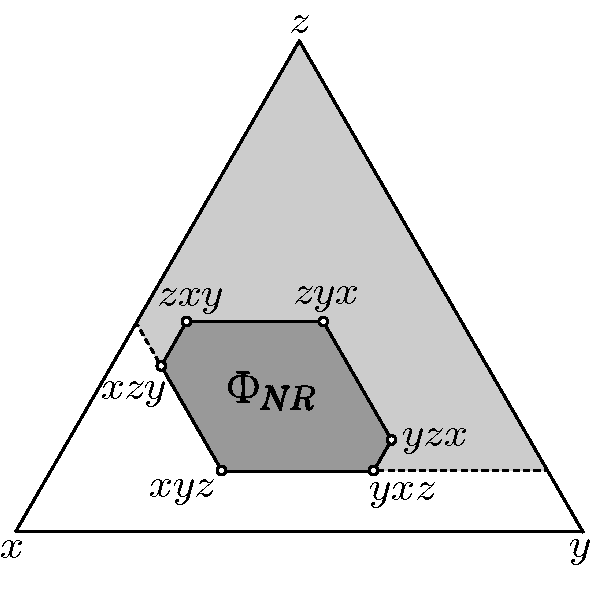
\includegraphics[width=2in]{graphics/ach/MNR_lotteries.pdf}
\end{center}
 

%\caption{In $\Delta(X)$, the lotteries stochastically dominated by the point $\varphi(\mu(\succsim))$ when $x\succ y \succ z$ (labeled $xyz$) are shown in light gray. The lotteries that are dominated by the truthful announcement for every $\succsim$ are shown in dark gray ($\Phi_{NR}$).}\label{fig:MNR_lotteries}
\end{figure}

Light gray: lotteries dominated by $\varphi(\mu(\succ))$ for $x\succ y\succ z$\\
Dark gray: lotteries dominated by $\varphi(\mu(\succ))$ for all possible $\succ$\\
So if $m\in M_{NR}$, pay something in $\Phi_{NR}$!!

\end{frame}


%%%%%%%%%%%%%%%%%%%%%%%%%%%%%%%%%%%%%%%%%%%%%%%%%%%%%%%%%%%%%%%%%%%

\begin{frame}
  \frametitle{Characterization (Lotteries)}
\begin{theorem}
     $(D,\varphi)$ is incentive compatible w.r.t. $\mathcal{E}^\mathrm{mon}$ if and only if
    \begin{enumerate}
      \item $\varphi$ is a WSS mechanism;
      \item $\varphi$ satisfies switch positivity;
      \item if $m\in M_{NR}$ then $\varphi(m)\in conv(\varphi(M_R))\setminus\varphi(M_R)$.
    \end{enumerate}
\end{theorem}


\end{frame}

%%%%%%%%%%%%%%%%%%%%%%%%%%%%%%%%%%%%%%%%%%%%%%%%%%%%%%%%%%%%%%%%%%%%%

%%%%%%%%%%%%%%%%%%%%%%%%%%%%%%%%%%%%%%%%%%%%%%%%%%%%%%%%%%%%%%%%%%%%%
\begin{frame}
  \frametitle{`Proof'}

$D_1=\{x,y\},~ D_2=\{x,z\},~ D_3=\{y,z\}$

\bigskip
\bigskip

There is a normalized and convex `capacity' $v:2^{\{x,y,z\}} \rightarrow [0,1]$ that `represents' $\varphi$:
\begin{eqnarray*}
\varphi(\mu(\succsim))(a_1) &=& v(a_1,a_2,a_3)-v(a_2,a_3)\\
\varphi(\mu(\succsim))(a_2) &=& v(a_2,a_3)-v(a_3)\\
\varphi(\mu(\succsim))(a_3) &=& v(a_3)
\end{eqnarray*}
$\{a_1,a_2,a_3\}=\{x,y,z\}$ and $\succsim$ ranks $a_1\succsim a_2 \succsim a_3$.


\end{frame}


%%%%%%%%%%%%%%%%%%%%%%%%%%%%%%%%%%%%%%%%%%%%%%%%%%%%%%%%%%%%%%%%%%%%%
\begin{frame}
  \frametitle{`Proof' (cont.)}

%$D_1=\{x,y\},~ D_2=\{x,z\},~ D_3=\{y,z\}$
%
%\bigskip
%\bigskip

Each $v$ can be represented uniquely by the `unanimity capacities':
$$v(A) = \sum_{E\subseteq A} \lambda (E)$$


\begin{eqnarray*}
\varphi(\mu(\succsim))(a_1) &=& v(a_1,a_2,a_3)-v(a_2,a_3) = \sum_{a_1\in E} \lambda(E)\\
\varphi(\mu(\succsim))(a_2) &=& v(a_2,a_3)-v(a_3) = \sum_{a_2\in E\subseteq \{a_2,a_3\}} \lambda(E)\\
\varphi(\mu(\succsim))(a_3) &=& v(a_3) = \sum_{E\subseteq \{a_3\}} \lambda(E)
\end{eqnarray*}

But this is exactly the required representation...

\bigskip

\textbf{Note:} $v$ convex $\Leftrightarrow$ $\lambda$ satisfies ``switch positivity''

\end{frame}


%%%%%%%%%%%%%%%%%%%%%%%%%%%%%%%%%%%%%%%%%%%%%%%%%%%%


\begin{frame}
  \frametitle{IC Mechanisms: Acts vs. Lotteries}

\begin{itemize}
\item The lotteries framework can be seen as a restriction of the set of possible extensions $\succsim^*$

\item The subject is indifferent between any two acts that generate the same lottery

\item Incentive compatibility becomes a weaker requirement

\item `More' mechanisms are IC
\end{itemize}

\end{frame}


%%%%%%%%%%%%%%%%%%%%%%%%%%%%%%%%%%%%%%%%%%%%%%%%%%%%%%%%%%%%%%%%%%%

\begin{frame}
  \frametitle{IC Mechanisms: Acts vs. Lotteries}

Imagine the Savage framework with subjective belief $\mu$ on $\Omega$

\begin{definition}
Say that $((\Omega ,\mu), \phi)$ \emph{generates} $\varphi$ if, for each $m\in M$ and $x\in X$,
$$\varphi(m)(x) = \mu\left(\{\omega\in\Omega: \phi(m)(\omega)=x\}\right).$$
\end{definition}

\end{frame}


%%%%%%%%%%%%%%%%%%%%%%%%%%%%%%%%%%%%%%%%%%%%%%%%%%%%%%%%%%%%%%%%%%%%%%%%%%%%%%%%%%%%%


\begin{frame}
  \frametitle{IC Mechanisms: Acts vs. Lotteries}

\begin{proposition}
If $\phi$ is an IC act-mechanism (defined on some state space $\Omega$), and $\mu$ is a full-support probability distribution on $\Omega$, then the lotteries-mechanism $\varphi$ generated by $((\Omega ,\mu), \phi)$ is IC.
\end{proposition}

\begin{proposition}
Assume that $\varphi$ is an IC lotteries-mechanism.
\begin{enumerate}
\item If the associated weighting vector $\lambda$ of $\varphi$ is non-negative, then there exists an IC acts-mechanism $\phi$ (on some $\Omega$) and a probability $\mu$ on $\Omega$ such that $((\Omega, \mu), \phi)$ generates $\varphi$ on rationalizable messages.

\item If the associated weighting vector $\lambda$ of $\varphi$ contains negative elements, then $\varphi$ cannot be generated by any IC acts-mechanism $\phi$ (even when restricted to rationalizable messages).
\end{enumerate}
\end{proposition}


\end{frame}

\begin{frame}
  \frametitle{Summary}
  \begin{itemize}
    \item If paying all, need to assume no complementarities.
    \begin{itemize}
      \item Fairness, portfolio, hedging, wealth, ...
    \end{itemize}
    \item If RPS, need to assume monotonicity. Weak, unless 2-stage gambles.
    \begin{itemize}
      \item Reduction \& non-expected utility
      \item Order Reversal \& ambiguity aversion
    \end{itemize}
    \item Other mechanisms may be IC for certain models.
    \item \textbf{Experimenter needs to decide for themselves!}
  \end{itemize}

  \bigskip

  My (current) opinion:
  \begin{itemize}
    \item Use RPS
    \item Separate decisions as much as possible.
    \item Use separate, physical randomizing devices.
  \end{itemize}
\end{frame}

\begin{frame}
  \frametitle{Other Issues}
  Other Monotonicity Violations:
  \begin{itemize}
    \item Decision Overload w/ Easy/Default Option (NCaT also questionable)
    \item Ex-Ante Fairness (NCaT: ex-post fairness)
    \item Irrational Diversification (NCaT also violated)
    \item Repeated decision problems (randomization)
    \item List format (Brown-Healy)
  \end{itemize}

  \bigskip

  Issues Besides IC:
  \begin{itemize}
    \item Payment Inequality \& Variance (matching pennies)
    \item Payment Size ($1/k$; same for NCaT)
    \item Random Choice
  \end{itemize}
  \bigskip
\end{frame}


\begin{frame}
  \frametitle{}
  \begin{center}
    The End
  \end{center}
\end{frame}


%%%%%%%%%%%%%%%%%%%%%%%%%%%%%%%%%%%%%%%%%%%%%%%%%%%%%%%%%%%%%%%%%%%%%%%%%%%%%%%%%%%%%


%\begin{frame}
%  \frametitle{How Strong is Monotonicity?}
%
%\begin{center}
%    \begin{tabular}{|c||c|c|c|c|c|c|}
%      \hline
%                & \multicolumn{6}{|c|}{States of the World} \\ \hline
%      Act   & 1     & 2     & 3     & 4     & 5     & 6     \\ \hline\hline
%      $f$ & $\$1$ & $\$25$ & pizza & $\$0$ & $\$1$  & Twix \\ \hline
%      $g$ & $\$1$ & $\$24$ & pizza & $\$0$ & $\$1$  & Mars \\ \hline
%    \end{tabular}
%\end{center}
%
%\bigskip
%
%$\$25 \succ \$24$ and  Twix$\succ$Mars  $\Rightarrow f\succ^* g$
%
%\bigskip
%
%\begin{itemize}
%\item Seems quite innocent
%
%\item A fundamental axiom of decision theory
%
%\item May become strong when combined with other axioms...
%
%\end{itemize}
%
%\end{frame}
%
%%%%%%%%%%%%%%%%%%%%%%%%%%%%%%%%%%%%%%%%%%%%%%%%%%%%%%%%%%%%%%%%%%%%%%%%%%%%%%%%%%%%%%
%
%
%\begin{frame}
%  \frametitle{Back to the Problematic Example}
% Let $L=(0.5,\$0;0.5,\$3)$.
%  \begin{itemize}
%    \item Decision 1: $L$ vs. \$1 for sure
%    \item Decision 2: $L$ vs. \$2 for sure
%    \item Each decision chosen for payment w/ 50\% probability
%  \end{itemize}
%
%  \bigskip
%
%  \begin{itemize}
%    \item Suppose $\$2\succ L \succ \$1$
%    \item Picking $\{L,\$2\}$ gives lottery $(0.25,\$0;0.5,\$2;0.25,\$3)$ (TRUTH)
%    \item Picking $\{\$1,\$2\}$ gives lottery $(0.5,\$1;0.5,\$2)$ (LIE)
%    \item $\exists$ rank-dependent utility preferences where $\$2\succ L \succ \$1$ and LIE $\succ$ TRUTH
%  \end{itemize}
%  $$
%        U(f) = \sum_{s=1}^n u(x_s)\left[ q(\sum_{r=1}^s p_r) - q(\sum_{r=1}^{s-1} p_r) \right]
%  $$
%
%\end{frame}
%
%%%%%%%%%%%%%%%%%%%%%%%%%%%%%%%%%%%%%%%%%%%%%%%%%%%%%%%%%%%%%%%%%%%%%%%%%%%%%%%%%%%%%%
%
%
%\begin{frame}
%  \frametitle{Current Practice}
%  Payment mechanisms used in experimental papers published in 2011:
%
%  \bigskip
%
%  \begin{center}
%\begin{tabular}{r||c|c|c|c||c|c||c}
%                             & \multicolumn{7}{c}{Payment Mechanism} \\
%                             \hline
%                             & No  &     &  Some   & Pay    & Other & Single    &       \\
%Journals                     & Pay & RPS & Random  & All    & Mech. & Decision & Total \\
%\hline
%Top 5               &  0   & 4   &  0      & \textbf{13}  &  0        &  13        & 30    \\
%\emph{ExpEcon}   &  1   & 4   &  3      & \textbf{8}  &  1       &  10        & 27
%\end{tabular}
%\end{center}
%
%\end{frame}
%
%
%\begin{frame}
%  \frametitle{Possible Issues}
%  \textbf{Decision Overload}
%  ``With 50 decisions, $Pr(D_i)\approx 2\%$!''\\
%   Subjects won't care.  aka `The Flat Maximum Critique'
%  \begin{itemize}
%    \item This would be a (plausible) violation of monotonicity.\\
%    \begin{tabular}{|c||c|c|c|c|c|c|}
%      \hline
%      Act   & 1     & 2     & 3     & 4     & $\cdots$     & 50     \\ \hline\hline
%      $\phi(x_1,x_2,x_3,\ldots,x_{50})$ & $x_1$ & $x_2$ & $x_3$ & $x_4$ & $\cdots$ & $x_k$ \\ \hline
%      $\phi(x_1,y_2,x_3,\ldots,x_{50})$ & $x_1$ & $y_2$ & $x_3$ & $x_4$ & $\cdots$ & $x_k$ \\ \hline
%    \end{tabular}\\
%    $\phi(x_1,x_2,x_3,\ldots,x_{50})\sim^*\phi(x_1,y_2,x_3,\ldots,x_{50})$
%    \item Perhaps $\exists$ default message $m^0$ that is `costless',\\
%          but truth $m^*$ may be `costly'.\\
%          Then $\phi(m^0)\succ^* \phi(m^*)$, IC fails.
%  \end{itemize}
%
%  \bigskip
%
%  But, no other mechanism is better.
%
%  \bigskip
%
%  Lesson: Don't try to squeeze 50 decisions out of a \$20 experiment!!
%
%\end{frame}

%\begin{frame}
%  \frametitle{Possible Issues}
%  \textbf{Ex-Ante Fairness}\\
%  Two binary \$10 dictator games, one with Alice, one with Bob.
%  \begin{itemize}
%    \item Subject prefers to keep \$10 in each
%    \begin{itemize}
%      \item Truth: $m^*=(\$10,\$10)$
%    \end{itemize}
%    \item But prefers lottery:
%    \begin{enumerate}
%      \item 50\%: \$10 to self
%      \item 50\%: \$10 to Bob
%    \end{enumerate}
%    \item Thus, $\phi(\$10,\$0)\succ^* \phi(m^*)$
%    \item Monotonicity violated.
%  \end{itemize}
%
%  \bigskip
%
%  Lesson: Avoid experiments where RPS can be used to be more `fair'
%\end{frame}

%\begin{frame}
%  \frametitle{Possible Issues}
%  \textbf{Non-EU \& Reduction of Compound Lotteries/Acts}\\
%  \begin{center}
%  $D=\{\{f,\$2\},\{g,\$2\}\}$. Suppose $\$2\succ f$ and $\$2\succ g$.\\
%    \begin{tabular}{c|cc}
%     Act & $H_1$ & $T_1$ \\
%    \hline
%     $f$ & \$4 & \$0 \\
%     $g$ & \$0 & \$4
%    \end{tabular}
%
%    \bigskip
%
%    \begin{tabular}{c||cc||cc|cc}
%    Msg        & $H_2$   & $T_2$  & $H_2\wedge H_1$ & $H_2\wedge T_1$ & $T_2\wedge H_1$ & $T_2\wedge T_1$ \\
%    \hline
%    $(f,g)$    &  $f$    & $g$   &     \$4          &     \$0        &   \$0           &   \$4          \\
%    $(\$2,\$2)$&  \$2    & \$2   &     \$2          &     \$2        &   \$2           &   \$2
%    \end{tabular}
%  \end{center}
%  \bigskip
%
%  Monotonicity: $(\$2,\$2)\succ (f,g)$. No longer related by dominance after reduction.
%
%\end{frame}


%\begin{frame}
%  \frametitle{Possible Issues}
%  \textbf{Extreme Risk Aversion}
%  \begin{itemize}
%    \item $D_1=\{\$10,\$9\}$
%    \item $D_2=\{\$9\}$
%    \item IC violated if $\$9 \succ^* (0.5,\$10;0.5,\$9)$
%    \item Another violation of monotonicity
%    \item No EU person would do this
%    \begin{itemize}
%      \item Nor RDU/Maxmin/Choquet/Prospect Theory/$\ldots$
%    \end{itemize}
%  \end{itemize}
%\end{frame}

%\begin{frame}
%  \frametitle{Possible Issues}
%  \textbf{Framing}
%  \begin{itemize}
%    \item $D_1=\{$Burger, Salad$\}$
%  \end{itemize}
%
%  \bigskip
%
%  \begin{itemize}
%    \item $D_1=\{$Burger, Salad$\}$
%    \item $D_2=\{\mathrm{Gym}_A,\mathrm{Gym}_B\}$
%  \end{itemize}
%
%  \bigskip
%
%  Here, $\succsim$ changes with $D$!\\
%  ``The Isolation Hypothesis'' (K\&T, Cox et al)
%  \begin{itemize}
%    \item Not a problem with mechanism
%    \item Problem with interpretation
%  \end{itemize}
%
%  \bigskip
%
%  Lesson: Be careful about generalizing results
%\end{frame}

%\begin{frame}
%  \frametitle{Possible Issues}
%  \textbf{Linked Decisions}
%  \begin{itemize}
%    \item Subjects play several repeated games
%    \begin{enumerate}
%      \item Pay for each period, or
%      \item pay for each repeated game?
%    \end{enumerate}
%    \item Strategy: function from histories to actions
%  \end{itemize}
%
%  \bigskip
%
%  Lesson: Carefully consider what constitutes a single `decision problem'
%\end{frame}

%\begin{frame}
%  \frametitle{Potential Issues}
%  \textbf{Decisions vs. Games}
%  \begin{itemize}
%    \item This paper: everything is an individual decision problem
%    \item Games \emph{can} be thought of as decision problems
%    \begin{itemize}
%      \item Players have types $\theta_i$
%      \item Types determine actions
%      \item Players are uncertain about others' types
%      \item Strategies are acts, mapping $\theta$ into outcomes\\
%      \begin{tabular}{|c|c|c|}
%      \hline
%                & L         & R         \\ \hline
%        U       & \$1,\$1   & \$0,\$0   \\ \hline
%        D       & \$0,\$0   & \$1,\$1   \\ \hline
%      \end{tabular}
%      \item Subjects have preferences over these acts\\
%            $U\succsim D$
%      \item RPS: acts over acts
%    \end{itemize}
%    \item Caution: Might be more complex than that.
%  \end{itemize}
%\end{frame}

%\begin{frame}
%  \frametitle{Lotteries Over Lotteries}
%  \begin{itemize}
%  \item Preference reversal literature
%  \begin{itemize}
%    \item $P$-bet $\succsim$ \$-bet, but $v(P$-bet$)<v($\$-bet$)$
%    \item Holt's (1986) rationalization:\\
%            Assumes reduction of compound lotteries. Shows RPS is IC only if independence axiom satisfied.\\
%            Thus, reversals are `just' a violation of independence.
%    \item Segal's (1988) rationalization:\\
%            Assumes independence. Shows RPS is IC only if reduction axiom is satisfied.\\
%            Thus, reversals are `just' a violation of reduction.
%    \item Starmer \& Sugden, Karni \& Saffra, Cox et al., Swarthout \& Harrison
%  \end{itemize}
%  \item Previous literature: $X=\Delta(\mathbb{R})$\\
%  \item RPS: $\Delta(\Delta(\mathbb{R}))$\\
%  \item Much more structure than our paper
%  \end{itemize}
%\end{frame}

%\begin{frame}
%  \frametitle{How We Fit}
%  \begin{itemize}
%    \item Two-stage lotteries
%    \item `Upper-stage': RPS mechanism
%    \item `Lower-stage': chosen lotteries
%    \item Monotonicity for IC = upper-stage monotonicity
%  \end{itemize}
%\end{frame}

%\begin{frame}
%  \frametitle{Monotonicity \& IC}
%  \textbf{Fact:} Upper-stage monotonicity + reduction $\Rightarrow$ lower-stage independence
%  \begin{itemize}
%    \item Suppose $f \succ g$
%    \item Consider $(p,f;1-p,h)$ vs. $(p,g;1-p,h)$
%    \item Monotonicity: $(p,f;1-p,h) \succ (p,g;1-p,h)$
%    \item Reduction: $pf+(1-p)h \succ pg+(1-p)h$
%    \item Thus, lower-stage independence!
%  \end{itemize}
%
%  \bigskip
%
%  \begin{enumerate}
%    \item If you believe in reduction, then IC requires$^*$ lower-stage EUT
%  \end{enumerate}
%\end{frame}

%\begin{frame}
%  \frametitle{The Cox et al (2011) Experiment}
%  \begin{itemize}
%    \item $D_1 = \{A,B\}$
%    \item 17\% choose $A$
%  \end{itemize}
%
%  \bigskip
%
%  \begin{itemize}
%    \item $D_1 = \{A,B\}$, $D_2 = \{C,D\}$
%    \item 45\% choose $A$
%  \end{itemize}
%
%  \bigskip
%
%  \begin{itemize}
%    \item $D_1 = \{A,B\}$, $D_2 = \{E,F\}$
%    \item 21\% choose $A$
%  \end{itemize}
%
%  \bigskip
%
%  Clearly framing/menu effects.
%
%\end{frame}

%\begin{frame}
%  \frametitle{The Cox et al (2011) Experiment}
%  Either:
%  \begin{enumerate}
%    \item Reduction is satisfied and lower-stage independence fails\\
%          (Thus, monotonicity fails)
%    \item Reduction is not satisfied and monotonicity still fails
%    \item $\succsim$ depends on $D$
%  \end{enumerate}
%
%  \bigskip
%
%  None of these are great news.
%
%  \bigskip
%
%  Without monotonicity, we know \emph{nothing} about IC mechanisms.
%
%\end{frame}

%\begin{frame}
%  \frametitle{The Lotteries Case}
%  The more structure you put on the preferences, the larger the set of IC mechanisms.
%
%  \bigskip
%
%  Cox et al (2011): `Pay all correlated' mechanism IC for non-EU prefs w/ reduction
%
%  \bigskip
%
%  For $\Delta(X)$ ($X$ has no structure), we have a characterization.\\
%  $(D,\phi)$ IC $\iff$ $\phi$ is a certain generalization of RSS\\
%  (Not much bigger than RSS mechanisms)
%
%\end{frame}

%\begin{frame}
%  \frametitle{Lessons}
%  Recall: RPS = pay for 1 random problem\\
%  Our results:
%  \begin{enumerate}
%    \item RPS is IC if preferences are monotonic, EU, Prob. Sophisticated,...
%    \item If \emph{all} monotonic prefs admissible, RPS is essentially the \emph{only} IC mech
%    \begin{itemize}
%      \item Can pay using SI sets, but those seem rare in practice
%    \end{itemize}
%    \item If you \emph{must} pay for multiple decisions, assume NCaT
%    \item If you don't believe in monotonicity, only have 1 decision
%  \end{enumerate}
%
%  Warnings:
%  \begin{itemize}
%    \item Monotonicity can still be violated
%    \item Don't have too many decisions
%    \item Make sure a single `decision' is properly defined
%  \end{itemize}
%\end{frame}





\end{document}